\documentclass{../../../../res/univ-projet}
\usepackage[utf8]{inputenc}
\usepackage[francais]{babel}
\usepackage[T1]{fontenc}
\usepackage{graphicx}
\filiere{M1SSI}
\logo{../../../../res/logo_univ.png}

\author{Benjamin \bsc{Zigh}}
\title{Manuel d'Utilisation de l'Application OTPToken}
\signataire{Magali \bsc{Bardet}, Bruno \bsc{Macadré}}

\begin{document}

\maketitle
\newpage
\tableofcontents
\newpage

\section{Introduction}
\subsection{Présentation de l'application}

L'application \verb$OTPToken$ est une application permettant de générer des mots de passe à usage unique de type HOTP et TOTP, dans les respect des RFC 4226 et 6238. L'application est compatible avec tous les services d'authentification HOTP et TOTP respectant ces mêmes RFC.

\subsection{Licence GPL}
Cette application, ainsi que son code source, sont disponibles selon les termes de la licence GPL, accessible \href{http://opensource.org/licenses/GPL-3.0}{ici}.

\subsection{Pré-requis matériels}
L'application peut être installée sur tout téléphone \verb$Android$ dont la version du système est supérieure ou égale à \verb$2.3.x$\footnote{Une connexion internet peut être requise lors du premier lancement sur les versions inférieures à \verb?4.0?}

\section{Installation}
\subsection{Installation via USB}
L'installation via USB s'effectue en plusieurs étapes:
\newline
\begin{description}
\item[Étape 1:] Télécharger \verb$OTPToken.apk$ sur le site de l'application \verb$OTPToken$ sur un ordinateur.
\item[Étape 2:] Connecter le téléphone Android en USB pour accéder au stockage interne.
\item[Étape 3:] Copier le fichier \verb$OTPToken.apk$ sur la mémoire du téléphone.
\item[Étape 4:] Lancer le fichier \verb$OTPToken.apk$ et patienter le temps de l'installation.\footnote{Votre téléphone doit être configuré pour accepter l'installation de programmes provenant de sources externes. Veuillez vous référer à la documentation Android}
\end{description}

\subsection{Installation via Internet}
L'installation via Itnernet s'effectue en plusieurs étapes:
\newline
\begin{description}
\item[Étape 1:] Télécharger \verb$OTPToken.apk$ sur le site de l'application \verb$OTPToken$ sur votre téléphone.
\item[Étape 2:]  Lancer le fichier \verb$OTPToken.apk$ et patienter le temps de l'installation. \footnotemark[\value{footnote}]
\end{description}
\newpage

\section{Utilisation}
\subsection{Première utilisation}
\subsubsection{Création du code PIN}
Lors du premier lancement, il est nécessaire de fournir un code PIN qui sera utilisé pour sécuriser l'accès à l'application.

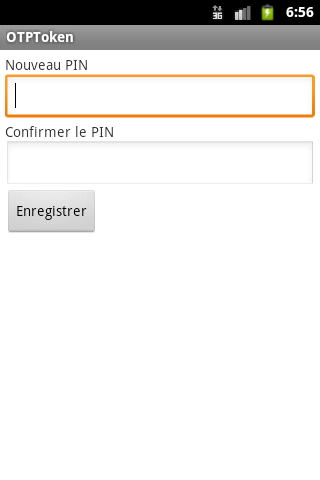
\includegraphics[scale=0.5]{enterpin.png}


\subsubsection{Création du premier OTP}
Une fois un code PIN choisi, on accède à la création du premier OTP.

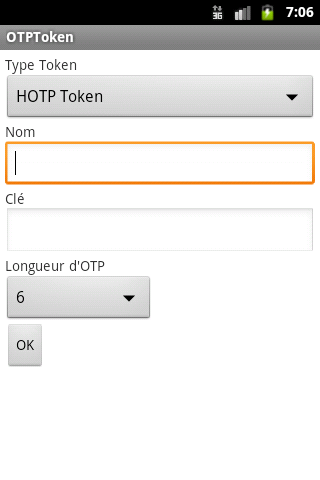
\includegraphics[scale=0.5]{firstotp.png}

\subsection{Génération d'un OTP}
On génére un OTP simplement en appuyant sur la ligne correspondant à l'OTP souhaité.

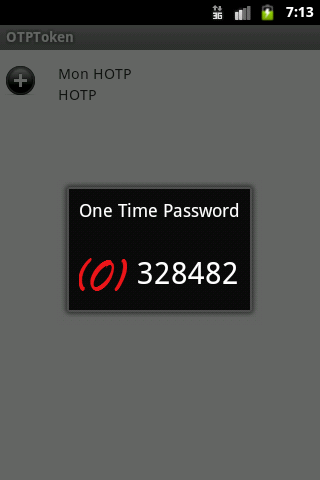
\includegraphics[scale=0.5]{genotp.png}

\subsection{Menu}
En appuyant sur la touche menu du téléphone, on accède au menu permettant d'ajouter ou de supprimer un OTP enregistré, de changer son code PIN, et de resynchroniser l'horloge\footnote{Cette fonctionnalité n'est à utiliser qu'en cas de problème d'authentification en TOTP}

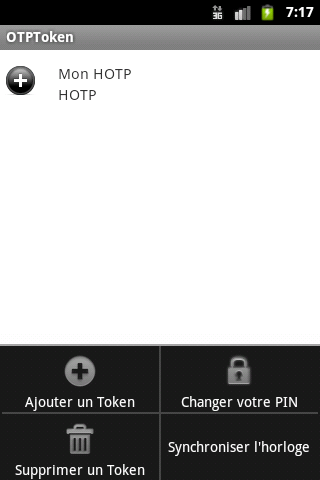
\includegraphics[scale=0.5]{menu.png}

\end{document}